\section{Round Scheduling}
\label{sect:scheduling}
The simplest way to take advantage of the efficiency of batch processing is to
schedule all the work to be done in one round.  This works well if all of the
data being backed up are only copies, e.g. a separate backup system which data
is sent to over the network. However, in our case we are backing up the
original virtual disk, so a single round backup presents several problems.
The first is that the average turnaround time for a VM is the time it takes to
backup all the VMs. The second, which is related to the first, is that a single
round backup has the highest cost to maintain a consistent view of the virtual
disks. We use Copy on Write (CoW) for this, and the consistent view must be
maintained between stage 1a and stage 2b, which can have sisgnificant cost if
the system must wait for every single VM before unlocking any of the VMs.
Other studies have
shown that as much as 8\% or even more of total capacity must be reserved for
CoW \cite{EMCIncrementalDataChanges}. The actual cost of CoW is a factor of the
data size, the write rate, and duration CoW is taking place. The data size
isn't something we can change, nor the write rate, but we can minimize the
duration that a given VM is undergoing CoW. By minimizing the backup time for
individual VMs we also improve CoW cost. To evaulate our
CoW cost improvement, we assume a poisson distribution of
writes (which closely fits the meaured results from
\cite{EMCIncrementalDataChanges}).

Our basic CoW cost model is:
\[
    CoW=n(1-e^{-m/n})
\]
    where
\[
    m=tw(1-d_1)c
\]

In the above model, $n$ is the number of dirty segments, $t$ is the time under
CoW, $w$ is the
write rate during CoW, $d_1$ is the \% of clean data (which doesn't go under
CoW), and $c$ is a constant determining how likely writes are to touch dirty
segments which haven't yet been copied vs. dirty segments which have already
been copied during the current backup. With this CoW cost model and the earlier
performance model, we can estimate the CoW cost of a given backup schedule.
Note that CoW ends in Stage 2b, so only the time up to the end of 2b counts
towards CoW. \todo{we still need to pick a value for $c$}

In addition to backup time for individual VMs, another cost consideration is
total backup time for the system. It is generally preferred to run backups
during low demand hours to make use of otherwise unused time and minimize the
impact on users. This leaves a window of several hours (e.g. from 1am to 4am)
to complete the backup. The more rounds there
are the shorter each round can be and therefore the smaller the VM backup times
and the total CoW costs. The
more rounds there are however the greater the overheads and some of the
efficiency gained from batch processing is lessened. We balance these costs by
developing an algorithm to schedule VMs into rounds.

From our requirements a model that closely fits our goals is the dual version
of the
bin packing problem. In standard bin packing the goal is to fit all of the
items into as few bins as possible, without overfilling any bins. In the dual
version of the problem however as many bins as possible are to filled to at
least some minimum level. This fits our purpose because we want to maximize the
number of rounds to minimize VM backup times, with some constraint to keep the
efficiency benefits of batch processing and keep the total backup time low.
In our dual-bin-packing solution the constraint is to keep the total
cost of the schedule under a time limit rather than mandating a minimum bin
level. We have adapted
an algorithm for dual bin packing\cite{DualBinPacking} to fit our VM
scheduling problem. The algorithm adapted is called iterated A and works by
iteratively callng a bin packing heuristic A with the items to be scheduled and
the number of bins, using binary search to arrive at the best number of
bins. A(I,N) is defined to return the optimality of packing set I into N bins
using A. We take this basic idea and look at several VM packing heuristics to
arrive at an efficient packing algorithm. More formally, our adaptation of the
iterated A algorithm is defined as:


%lstset{basicstyle=\ttfamily\tiny
%}
\todo{justify choice of initial UB (right now it is mostly arbitrary)}
\begin{figure}
\begin{lstlisting}[frame=single]
Iterated A:
Set UB=min(n,2*v)
Set LB=1
while UB>LB
  set N = (UB+LB+1)/2
  if A(machines,N) > T, set UB=N-1
  else set LB=N
Halt
\end{lstlisting}
\caption{Iterated A scheduling algorithm, requires good choice of A to be effective}
\end{figure}

where A(machines,N) returns the total backup time of the schedule for N rounds\\
This algorithm returns the packing generated by A(machines,UB) after loop finishes

The general algorithm relies on a good choice of A to arrive at an efficent
packing. Our first VM packing heuristic, A0, is a na\"\i{}ve approach very
close to the un-adapted algorithm from the dual bin packing paper. For both
algorithms we develop, in case of ties, choose the left-most item.

\begin{figure}
\begin{lstlisting}[frame=single]
A0:
sort VMs in descending order by size
while there is an unscheduled VM
  pick the first unscheduled VM a
    pick the round with the current
    lowest runtime b
  schedule VM a to round b
Halt
\end{lstlisting}
\caption{Na\"{\i}ve round packing heuristic based on VM size and current round runtime}
\end{figure}

\begin{figure}[thb]
\centering
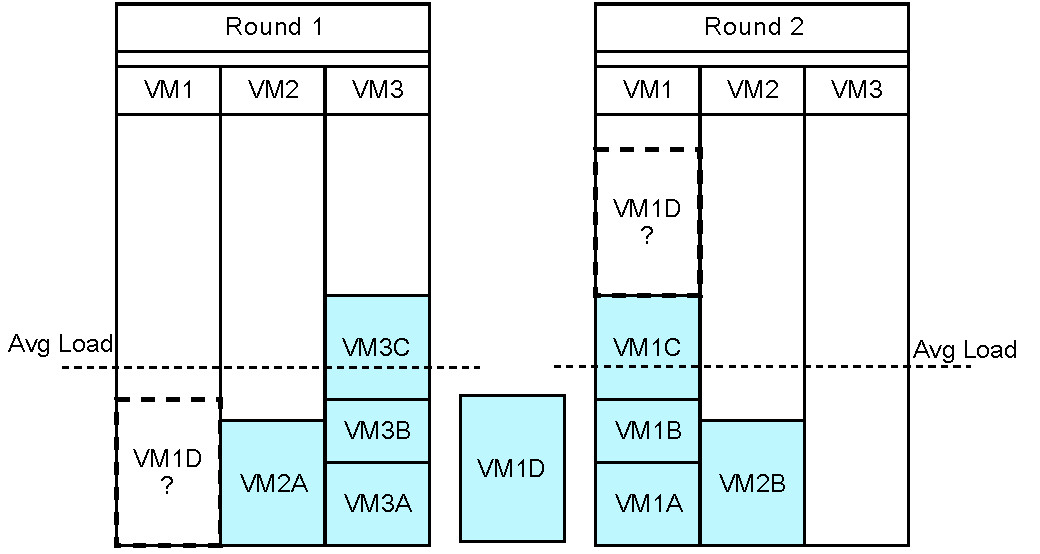
\includegraphics[width=0.5\textwidth]{images/VMRound.pdf}
\caption{Choosing a round to schedule a VM to. Though the rounds look
identical in terms of total/average load, Round 1 is a much better choice.}
\label{fig:VMRound}
\end{figure}

A0 does provide for shorter rounds (see Table~\ref{tab:schedule-costs}), but
the efficiency of the packing is poor due to several issues
The first issue is that the round with the current lowest runtime
is chosen. Because backup time is dependent on a combination of the highest
machine load and average machine load, if we add a VM to the currently most
loaded machine in a round it will increase runtime much more than if we add the
VM to a different round where that machine is currently empty. You can see this
in Figure~\ref{fig:VMRound}, where VM1D must be scheduled to one of two rounds
which currently have the same average/total load. The effect of VM1D on round 1
would be much less than the effect on round 2 because we wouldn't be increasing
the maximum machine load of the round, so we should schedule to round 1.
Therefore a better
scheduling heuristic is one based on predicted runtime after adding the VM, and
picking the round with the lowest runtime after adding the VM to that round.
This new round picking heuristic
takes into account that the same VM might have different affects on different
rounds. This aspect of round picking must be considered because we assume a VM
must be backed
up by the machine that hosts it. If the VMs are located on a DFS such that they
can be
backed up by any machine in the cluster then the problem of load balancing
becomes a simpler but much different problem, but isn't considered here. We
also pick the most heavily loaded (i.e. most data remaing) machine in case of
ties so we can make the most backup progress in a round, given equivalent
equivalent options.

Another improvement we can make to A0 is to the VM picking heuristic. For the
same reason as given above, the largest VM may not always have the greatest
impact on time (e.g. picking a slightly smaller VM on the most heavily loaded
machine has a greater impact than selecting the largest VM on a lightly loaded
machine). Our improved hueristic to pick VMs is to predict the one-round
runtime after removing that VM, and pick the VM whose removal most
decreases the single round time (i.e. the VM that has the greatest impact on
overall backup time). By picking VMs this way we take into account
the machine load in picking which VM to schedule next, and minimize the time
the remaining VMs will take to backup

After making the two above changes we arrive at VM packing heuristic A1.

\begin{figure}
\begin{lstlisting}[frame=single]
A1:
while there is an unscheduled VM
  pick the VM a whose removal will
    most decrease single round time
    tie-breaker:VM on most heavily
    loaded round
  pick the round b whose runtime will
    be lowest after adding VM a
  schedule VM a to round b
Halt
\end{lstlisting}
\caption{More effective round packing heuristic based on minimizing remaining work and predicted round time}
\end{figure}

A1 significantly improves our simulated results, also bringing our CoW costs
much closer to the best case than the worst case, as can be seen in
Figure~\ref{tab:schedule-costs}.  Our current implementation of the algorithm
focuses on the deduplication and so doesn't make use of CoW, but we can see
that our simulated times closely match measured runtimes (hopefully). \todo{I
haven't actually implemented the schedulers into the dedup yet to test this}
